\section{Dataset Imputation and Reclassification}
\subsection{Dataset Imputation and Justification}
The dataset given with this assignment has several missing values in it, namely 46 (7\%) in \textit{Reason\_for\_absence} and 3 (\textless 0.5\%) in \textit{Month\_of\_absence}. There are a number of ways to classify missing values, namely, MCAR or Missing Completely At Random (there is no relationship between the fact a value is missing and the rest of the instance), MAR or Missing at Random (there is a relationship between which values are missing and the rest of their instances but not what the value is) and MNAR or Missing Not At Random (the values which are missing and their actual value are linked to their instances). 

I imported the dataset into R \cite{langR} so I could analyse the data (using the package \cite{packfarff}). If the \textit{Reason\_of\_absence} was MCAR the distribution of each feature for both missing and non-missing reasons would be the same, however we see this is not the case (for conciseness only a few examples are given here, however all the plots made can be found in the appendices, plots were made with \cite{packggplot2}). As can be observed there is a vast difference between the distributions of each feature depending on if there's an associated reason for the absence. 

\begin{figure}[h]
\centering
\begin{minipage}{.5\textwidth}
  \centering
  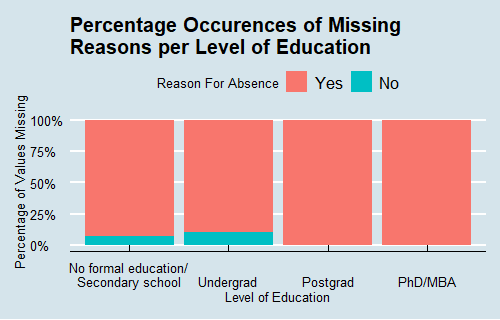
\includegraphics[width=.9\linewidth]{images/plot_missing_edu.png}
  \label{fig:plot_missing_edu}
\end{minipage}%
\begin{minipage}{.5\textwidth}
  \centering
  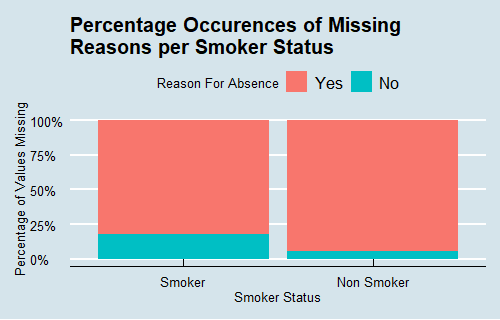
\includegraphics[width=.9\linewidth]{images/plot_missing_smoker.png}
  \label{fig:plot_missing_smoker}
\end{minipage}
\end{figure}

\begin{figure}[h]
\centering
\begin{minipage}{.5\textwidth}
  \centering
  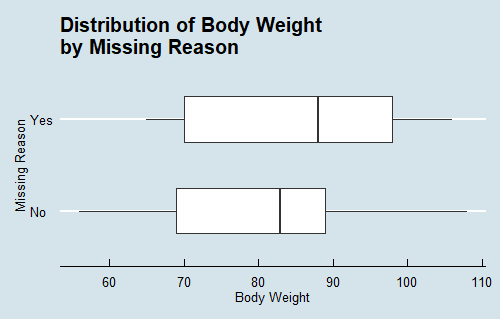
\includegraphics[width=.9\linewidth]{images/plot_dist_weight.png}
  \label{fig:plot_dist_weight}
\end{minipage}%
\begin{minipage}{.5\textwidth}
  \centering
  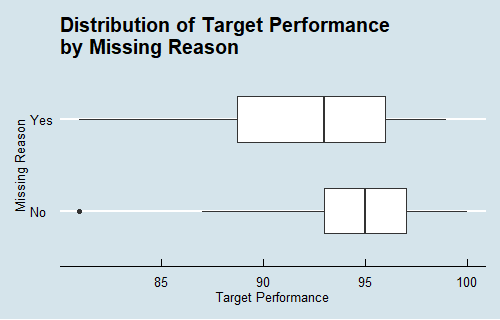
\includegraphics[width=.9\linewidth]{images/plot_dist_perf.png}
  \label{fig:plot_dist_perf}
\end{minipage}

\caption{Some plots to show that missing reasons is MAR}
\end{figure}

The fact that the missing data is not MCAR, it represents a significant proportion of our dataset and removing it would change the distributions of our features, we must therefore impute the data \cite{cheema2014}. Given the data was already R, I used a package called mice (Multivariate Imputation by Chained Equations) \cite{packmice}. mice works by replacing each variable with a starting replacement (usually the mean or mode) it then using all of the other variables to impute each column one by one, replacing those values that were originally missing, the idea being that after many rounds of this the values will converge together \cite{azur2011}. 

There were several reasons for using a MICE approach, namely, it works with MAR data as we proved was the case, it respects the existing variance of the features unlike a mean or mode replacement (such as what WEKA's filters use) and it works with categorical data unlike most imputation methods. However it should be acknowledged that MICE has flaws, for example, research has yet to be done on the best number of iterations to perform and there is no mathematical basis to this method of imputation unlike other methods.

\subsection{Reclassification and Re-Evaluation}
After imputation next was to reclassify on the new data and compare against the old classifiers. I loaded the .arff file into WEKA and retrained the same three classifiers, NaiveBayes, J48 and RandomForest. Again we will compare their F1 measures and ROC scores, the better of the two being marked in bold.

\begin{center}
\begin{tabular}{|r|l|l|l|l|}
\hline 
Classifier & \multicolumn{2}{l|}{F1 Measure} & \multicolumn{2}{l|}{ROC Score} \\ 
\hline 
 & Old & New & Old & New \\ 
\hline 
NaiveBayes & 0.549 & \textbf{0.554} & 0.782 & \textbf{0.784} \\ 
\hline 
J48 & \textbf{0.718} & 0.698 & \textbf{0.854} & 0.847 \\ 
\hline 
RandomForest & \textbf{0.788} & 0.751 & \textbf{0.934} & 0.858 \\
\hline 
\end{tabular}
\end{center}

Interestingly, and personally unexpectedly, we can see that NaiveBayes did slightly better (though really negligibly so) whereas J48 did slightly worse and RandomForest even more so. Most likely this is due to faults in the imputation method, maybe some features should have been excluded from contributing towards the imputation and the method of making the models could have been wrong too, here mice used multinomial logistic regression but maybe another method would be more appropriate. Of course the possibility can't be ignored that this method of imputation was inappropriate too, maybe training a classifier on complete case data and using it to find the missing values would have worked better. 